% ============================================================
%  NAND gate - breadboard wiring diagram (COMPLEMENTARY / CMOS-style).
%  Four transistors:  Q1,Q2 = 2N3904 (NPN) in series (pull-down);
%                      Q3,Q4 = 2N3906 (PNP) in parallel (pull-up).
%  Each input drives one NPN and one PNP through its own base resistor.
%  Tall layout: long leads, the bottom resistors/LEDs have clear margin.
%  Colour-coded jumper wires (see the legend); each column of five
%  holes in a bank is one node.
%  Compile:  pdflatex wiring.tex
% ============================================================
\documentclass[border=16pt]{standalone}
\usepackage{circuitikz}
\usepackage{tikz}
\usetikzlibrary{calc, positioning}

\definecolor{vcc}{RGB}{205,45,45}
\definecolor{gnd}{RGB}{35,35,40}
\definecolor{anet}{RGB}{20,140,60}
\definecolor{bnet}{RGB}{225,120,0}
\definecolor{onet}{RGB}{120,45,175}
\definecolor{mnet}{RGB}{120,90,60}
\definecolor{board}{RGB}{246,241,229}

\newcommand{\trans}[3]{%
  \pgfmathsetmacro\xe{0.7*#1}%
  \pgfmathsetmacro\xb{0.7*(#1+2)}%
  \pgfmathsetmacro\xc{0.7*(#1+4)}%
  \draw[fill=black!10]
        (\xe-0.4,9.55) -- (\xe-0.4,9.95)
        arc (180:0:{(\xc-\xe+0.8)/2} and 0.45) -- (\xc+0.4,9.55) -- cycle;
  \node[font=\footnotesize\bfseries] at (\xb,9.85) {#3};
  \node[font=\scriptsize,anchor=east] at (\xe-0.5,9.9) {#2};
  \draw (\xe,9.55)--(\xe,9.0);
  \draw (\xb,9.55)--(\xb,9.0);
  \draw (\xc,9.55)--(\xc,9.0);
  \node[red,font=\scriptsize\bfseries,anchor=east] at (\xe-0.16,8.78) {E};
  \node[red,font=\scriptsize\bfseries,anchor=east] at (\xb-0.16,8.78) {B};
  \node[red,font=\scriptsize\bfseries,anchor=east] at (\xc-0.16,8.78) {C};
}

\begin{document}
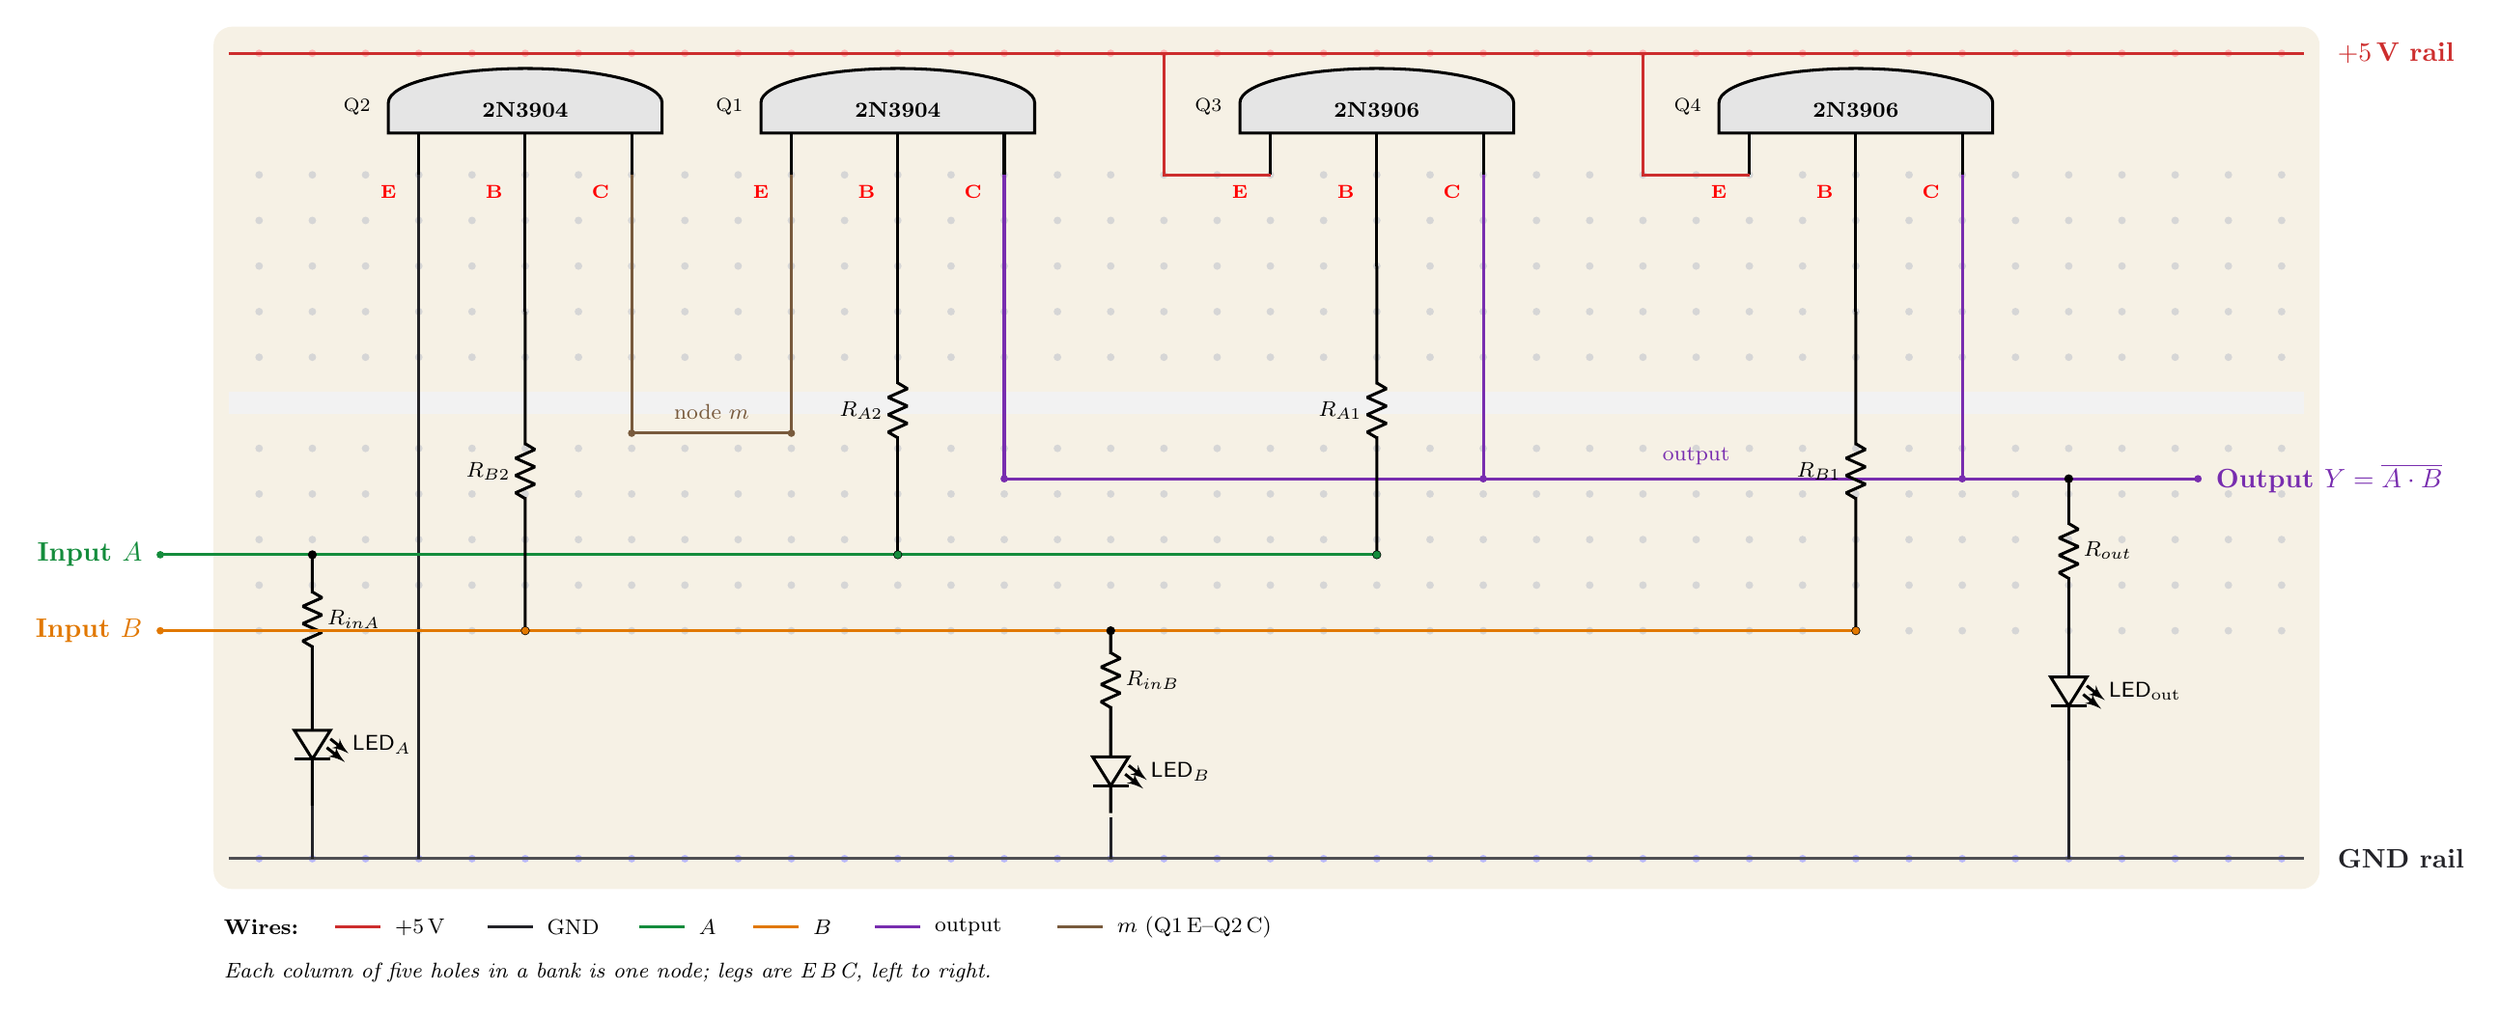
\begin{tikzpicture}[line width=1.1pt, font=\sffamily]
  \ctikzset{bipoles/thickness=1, bipoles/length=0.95cm, resistors/scale=0.9}

  % ---------- board (tall) ----------
  \fill[board,rounded corners=7pt] (0.1,-0.4) rectangle (27.8,10.95);
  \foreach \c in {1,...,39}{
    \foreach \y in {9.0,8.4,7.8,7.2,6.6, 5.4,4.8,4.2,3.6,3.0}{
      \fill[black!16] ({0.7*\c},\y) circle (0.5mm);}}
  \fill[black!5] (0.3,5.85) rectangle (27.6,6.15);
  \foreach \c in {1,...,39}{
    \fill[red!28]  ({0.7*\c},10.6) circle (0.5mm);
    \fill[blue!28] ({0.7*\c},0.0)  circle (0.5mm);}
  \draw[vcc]    (0.3,10.6) -- (27.6,10.6);
  \draw[gnd!80] (0.3,0.0)  -- (27.6,0.0);
  \node[vcc,font=\bfseries,anchor=west] at (27.9,10.6) {$+5\,$V rail};
  \node[gnd,font=\bfseries,anchor=west] at (27.9,0.0)  {GND rail};

  % ---------- transistors:  Q2,Q1 (NPN series) | Q3,Q4 (PNP parallel) ----------
  \trans{4}{Q2}{2N3904}
  \trans{11}{Q1}{2N3904}
  \trans{20}{Q3}{2N3906}
  \trans{29}{Q4}{2N3906}

  % ===== GND: Q2 emitter (col4) =====
  \draw[gnd] ({0.7*4},9.0) -- ({0.7*4},0.0);

  % ===== series link m: Q1 emitter (col11) <-> Q2 collector (col8) =====
  \draw[mnet] ({0.7*8},9.0)  -- ({0.7*8},5.6);
  \draw[mnet] ({0.7*11},9.0) -- ({0.7*11},5.6);
  \draw[mnet] ({0.7*8},5.6)  -- ({0.7*11},5.6);
  \fill[mnet] ({0.7*8},5.6) circle (1.4pt); \fill[mnet] ({0.7*11},5.6) circle (1.4pt);
  \node[mnet,font=\footnotesize,anchor=south] at ({0.7*9.5},5.65) {node $m$};

  % ===== +5 V: Q3, Q4 emitters (cols 20, 29) =====
  \draw[vcc] ({0.7*20},9.0) -- ({0.7*18},9.0) -- ({0.7*18},10.6);
  \draw[vcc] ({0.7*29},9.0) -- ({0.7*27},9.0) -- ({0.7*27},10.6);

  % ===== OUTPUT (violet): Q1.C(15) + Q3.C(24) + Q4.C(33) =====
  \draw[onet] ({0.7*15},9.0) -- ({0.7*15},5.0);
  \draw[onet] ({0.7*24},9.0) -- ({0.7*24},5.0);
  \draw[onet] ({0.7*33},9.0) -- ({0.7*33},5.0);
  \draw[onet] ({0.7*15},5.0) -- (26.2,5.0);
  \foreach \c in {15,24,33}{\fill[onet] ({0.7*\c},5.0) circle (1.4pt);}
  \node[onet,font=\footnotesize,anchor=south] at ({0.7*28},5.05) {output};
  \node[onet,anchor=west,font=\bfseries] at (26.3,5.0) {Output $Y=\overline{A\cdot B}$};
  \fill[onet] (26.2,5.0) circle (1.4pt);

  % ===== INPUT A (green): R_A2->Q1.B(13), R_A1->Q3.B(22), LED on col2 =====
  \draw[anet] (-0.6,4.0) -- ({0.7*22},4.0);
  \node[anet,anchor=east,font=\bfseries] at (-0.7,4.0) {Input $A$};
  \fill[anet] (-0.6,4.0) circle (1.4pt);
  \draw ({0.7*13},9.0)--({0.7*13},7.8); \draw ({0.7*13},7.8) to[R, l_=\footnotesize $R_{A2}$, -*] ({0.7*13},4.0);
  \draw ({0.7*22},9.0)--({0.7*22},7.8); \draw ({0.7*22},7.8) to[R, l_=\footnotesize $R_{A1}$, -*] ({0.7*22},4.0);
  \fill[anet] ({0.7*13},4.0) circle (1.4pt); \fill[anet] ({0.7*22},4.0) circle (1.4pt);
  \fill[anet] ({0.7*2},4.0) circle (1.4pt);
  \draw ({0.7*2},4.0) to[R, l=\footnotesize $R_{inA}$, *-] ({0.7*2},2.3);
  \draw ({0.7*2},2.3) to[leD, l=\footnotesize LED$_A$] ({0.7*2},0.7);
  \draw[gnd] ({0.7*2},0.7) -- ({0.7*2},0.0);

  % ===== INPUT B (orange): R_B2->Q2.B(6), R_B1->Q4.B(31), LED on col17 =====
  \draw[bnet] (-0.6,3.0) -- ({0.7*31},3.0);
  \node[bnet,anchor=east,font=\bfseries] at (-0.7,3.0) {Input $B$};
  \fill[bnet] (-0.6,3.0) circle (1.4pt);
  \draw ({0.7*6},9.0)--({0.7*6},7.2);  \draw ({0.7*6},7.2) to[R, l_=\footnotesize $R_{B2}$, -*] ({0.7*6},3.0);
  \draw ({0.7*31},9.0)--({0.7*31},7.2); \draw ({0.7*31},7.2) to[R, l_=\footnotesize $R_{B1}$, -*] ({0.7*31},3.0);
  \fill[bnet] ({0.7*6},3.0) circle (1.4pt); \fill[bnet] ({0.7*31},3.0) circle (1.4pt);
  \fill[bnet] ({0.7*17},3.0) circle (1.4pt);
  \draw ({0.7*17},3.0) to[R, l=\footnotesize $R_{inB}$, *-] ({0.7*17},1.7);
  \draw ({0.7*17},1.7) to[leD, l=\footnotesize LED$_B$] ({0.7*17},0.6);
  \draw[gnd] ({0.7*17},0.55) -- ({0.7*17},0.0);

  % ===== OUTPUT LED (col35) =====
  \fill[onet] ({0.7*35},5.0) circle (1.4pt);
  \draw ({0.7*35},5.0) to[R, l=\footnotesize $R_{out}$, *-] ({0.7*35},3.1);
  \draw ({0.7*35},3.1) to[leD, l=\footnotesize LED$_{\mathrm{out}}$] ({0.7*35},1.3);
  \draw[gnd] ({0.7*35},1.3) -- ({0.7*35},0.0);

  % ---------- legend ----------
  \begin{scope}[shift={(0.3,-1.4)}]
    \node[anchor=west,font=\footnotesize\bfseries] at (-0.2,0.5) {Wires:};
    \draw[vcc]  (1.4,0.5)--(2.0,0.5);  \node[anchor=west,font=\footnotesize] at (2.05,0.5){+5\,V};
    \draw[gnd]  (3.4,0.5)--(4.0,0.5);  \node[anchor=west,font=\footnotesize] at (4.05,0.5){GND};
    \draw[anet] (5.4,0.5)--(6.0,0.5);  \node[anchor=west,font=\footnotesize] at (6.05,0.5){$A$};
    \draw[bnet] (6.9,0.5)--(7.5,0.5);  \node[anchor=west,font=\footnotesize] at (7.55,0.5){$B$};
    \draw[onet] (8.5,0.5)--(9.1,0.5);  \node[anchor=west,font=\footnotesize] at (9.15,0.5){output};
    \draw[mnet] (10.9,0.5)--(11.5,0.5);\node[anchor=west,font=\footnotesize] at (11.55,0.5){$m$ (Q1\,E--Q2\,C)};
    \node[anchor=west,font=\footnotesize\itshape] at (-0.2,-0.1)
        {Each column of five holes in a bank is one node; legs are E\,B\,C, left to right.};
  \end{scope}

\end{tikzpicture}
\end{document}
